%% question-10.tex
%%

%% ==============================
\subsection{Modélisation explicite d'un objectif}
\label{sec:question10}
%% ==============================

Le concept d'objectif est présenté à l'aide de la figure \ref{fig:objectif}. Un \emph{Objectif} est parent de 4 enfants : \emph{Neant} qui est l'objectif par défault. \emph{Combinable} qui est lui même parent de \emph{AllerVers}, \emph{Contourner} et \emph{Eviter}.
\emph{CollecterMax} et \emph{Combattre} sont les deux derniers enfants.
Les \emph{Objectif} sont réalisés par des règles qui possèdent des \emph{Reaction}.

\begin{figure}
	\centering
	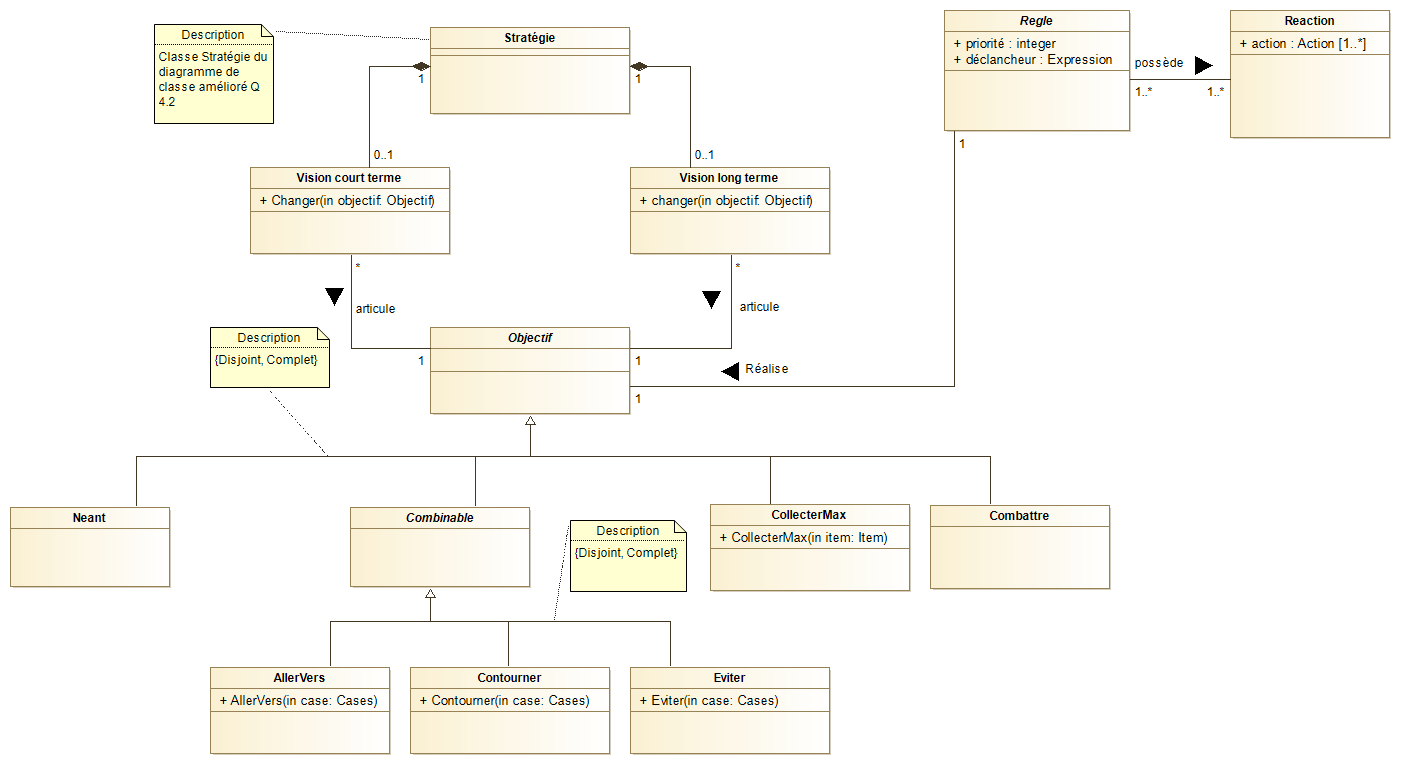
\includegraphics[width=500pt]{assets/class__Objectif}
	\caption{Diagramme de classe d'un objectif}
	\label{fig:objectif}
\end{figure}
